\documentclass[sigconf]{acmart}
% Cleaning 
\pagestyle{fancy} % removes running headers
\settopmatter{printacmref=false} % Removes citation information below abstract
\renewcommand\footnotetextcopyrightpermission[1]{} % removes footnote with conference information in first column
\pagestyle{plain} % removes running headers
\fancyhead{}
\settopmatter{printacmref=false, printfolios=false}
% Copyright
\setcopyright{none}
% \setcopyright{acmcopyright}
% \setcopyright{acmlicensed}
% \setcopyright{rightsretained}
% \setcopyright{usgov}
% \setcopyright{usgovmixed}
% \setcopyright{cagov}
% \setcopyright{cagovmixed}
\settopmatter{printacmref=false} % Removes citation information below abstract
\acmDOI{}

\usepackage{booktabs} % For formal tables
\usepackage{url}
\usepackage{algorithm}
\usepackage[noend]{algpseudocode}
\algtext*{EndWhile}% Remove "end while" text
\algtext*{EndIf}% Remove "end if" text
%\usepackage{flexisym}

\setlength{\parskip}{0pt}
\setlength{\parsep}{0pt}
\setlength{\headsep}{0pt}
\setlength{\topskip}{0pt}
\setlength{\topmargin}{0pt}
\setlength{\topsep}{0pt}
\setlength{\partopsep}{0pt}
%\linespread{0.95}
\usepackage{mdwlist}
\usepackage{amsmath}

\begin{document}
\title{\textit{Sample*} Diachronically Like-minded User Community Detection}\titlenote{Link to Github or an online repo}
\author{Ali Fani}
\affiliation{
  \institution{University of Windsor}
%   \streetaddress{P.O. Box 1212}
%   \city{Toronto} 
%   \state{ON} 
%   \country{Canada} 
%   \postcode{43017-6221}
}
\email{afani@uwindsor.ca}
\author{Hossein Fani}
% \authornotemark[1]
\orcid{0000-0002-6033-6564}
\affiliation{
 \institution{University of Windsor}
%   \city{Fredericton} 
%   \state{NB} 
%   \country{Canada} 
}\email{hfani@uwindsor.ca}

\begin{abstract}
{\color{blue}This is a \textit{sample} proposed method for your proposal. The sections and subsections are \textit{by no means} fixed and should be indeed changed or customized according to the proposal. }
\end{abstract}

\keywords{More Specific Keywords, Specific Keyword, General Keyword, More General Keyword}
\maketitle


\section{Problem Definition}
Our goal is to identify like-minded user communities whose members exhibit similar temporal dispositions towards similar topics. Here, we provide a formal statement of the problem after which we propose our approach in detail in the next section. We view the problem of like-minded user community detection as an instance of the set partitioning task on a set of users $\mathbb{U}$. A partition $\mathbb{P}$ of the set $\mathbb{U}$ of all users is a set of nonempty subsets of $\mathbb{U}$ as communities such that every user $u\in\mathbb{U}$ is in exactly one of these communities. Notationally, $\mathbb{P}= \{\mathbb{C}:\mathbb{C}\subseteq\mathbb{U},|\mathbb{C}|\geq 1\}$ such that $\forall\mathbb{C}_i,\mathbb{C}_{j\neq{i}}\in\mathbb{P}:\mathbb{C}_i\cap\mathbb{C}_j=\varnothing$ and $\bigcup_{\mathbb{C}\in\mathbb{P}}\mathbb{C}=\mathbb{U}$. Since we do not consider a set with one user as a community, we relax the partition definition by assuming $|\mathbb{C}|\geq2$ and drop the last union condition; i.e., $\mathbb{P}^*=\mathbb{P}\setminus\{\mathbb{C}:|\mathbb{C}|=1\}$. The goal of like-minded user community detection is to infer $\mathbb{P}^*$ such that highly similar users are in the same community $\mathbb{C}$, yet users of high dissimilarity are in different communities $\mathbb{C}_i$ and $\mathbb{C}_{j\neq{i}}$. In our work, we consider two users to be similar if they show similar temporal inclination towards a set $\mathbb{Z}$ of possible topics.

\section{Proposed Approach}\label{approach}
Our proposed like-minded community detection method seeks to find $\mathbb{P}^*$ with respect to the temporal topic-based sense of user similarity, defined in the previous section. The approach works through three pipelined phases: temporal topic-based user modeling, user vector representation (embedding), and user community detection. In the following, we describe the details of each step.

\subsection{Temporal Topic-based User Modeling}\label{topic_detection}
Our work relies on users' behavior towards a set of topics within time period $\text{T}$. To incorporate both users' topics of interest and temporality, for each user $u\in\mathbb{U}$, we model her inclination towards each topic $z\in\mathbb{Z}$ at each time interval $1\leq{t}\leq\text{L}$ through a matrix. The stacking of all user matrices will generate a cuboid denoted as \textit{points of temporal interest} (PoTI). An entry in PoTI shows how much a user $u\in\mathbb{U}$ is interested in a topic $z\in\mathbb{Z}$ in time interval $1\leq{t}\leq\text{L}$.

\begin{definition}
\textbf{Points of Temporal Interest (PoTI).} Let $\mathbb{U}$ be a set of users, $\mathbb{M}$ be the users' posts corpus, $\mathbb{Z}$ be a set of topics, and $\text{T}$ be a time period broken down into $\text{L}$ intervals, \textit{points of temporal interest} (PoTI) is a three dimensional matrix (cuboid) $\mathbb{U}\times\mathbb{Z}\times\text{T}= \{y^u_t[z]\}$ where $u\in\mathbb{U},z\in\mathbb{Z}$ and $1\leq{t}\leq\text{L}$ whose three dimensions correspond to users, topics and time intervals, respectively and the value $y^u_t[z]$ is the degree of u's interest in topic $z$ at time $t$.
\end{definition}

To instantiate PoTI, we need to find i) a set of topics that have been observed in time period $\text{T}$, i.e., $\mathbb{Z}$, and ii) each user's degree of interest at time $t$ towards each topic $z\in\mathbb{Z}$, i.e., $y^u_t[z]$. The set of possible topics can be derived by extracting the topics available in the collection of users' posts using various existing topic detection methods in the literature including topic modeling techniques such as latent Dirichlet allocation (LDA)~\cite{DBLP:journals/jmlr/BleiNJ03} as suggested in~\cite{DBLP:conf/ecir/ZarrinkalamFBK17, DBLP:conf/ecir/ZarrinkalamFBK16}. In order to identify the set of topics, ***.

\subsection{User Vector Representation (Embedding)}
The key contribution of this paper is to learn user vector representations from users' topics of interest with the expectation that temporally like-minded users end up closer to each other in the vector space. We hypothesize that an appropriate embedding method would bring significant performance into our main downstream task of like-minded user community detection compared to the state of the art. To build user embeddings, we first formally formulate what we mean by a like-minded pair of users. Then, we propose an embedding method which preserves pairwise like-minded proximity of the users through maximizing the likelihood that two like-minded users stay close to each other in vector space.

\subsubsection{User Like-minded Context Model}
In our approach, users would be considered to be like-minded if they share similar temporal and topical interest. More formally, the more two user $u_1$ and $u_2$ share instances of $y^{u_1}_t[z]\simeq{y^{u_2}_t[z]}$ in the PoTI for topics $z\in\mathbb{Z}$ across different time intervals $1\leq{t}\leq\text{L}$, the more similar they would be. 

\begin{definition}
  \textbf{Region of Like-mindedness (RoL).} A three-dimensional subspace of PoTI, such as $\text{R}$, is defined to be a region of like-mindedness (RoL) iff (i) all the values in this subspace are \textit{equal} with respect to a certain condition of homogeneity $c$; notationally, $\forall{y,y'}\in\text{R};c(y)=c(y')$ and (ii) it is \textit{maximal} such that there exists no other region of like-mindedness such as $\text{R'}$ which subsumes $\text{R}$.
\end{definition}

To find all regions of like-mindedness, RoLs, in PoTI, we adopt a similar strategy to~\cite{DBLP:conf/sigmod/ZhaoZ05} where subspace submatrices are mined from three-dimensional gene-sample-time gene expression microarrays. First, we find the RoLs in user and topic dimensions at each time interval. The output is two-dimensional (2-d) RoLs indexed by the time interval $1\leq{t}\leq\text{L}$, i.e., $\text{RoL}_t$. Then, we merge $\text{RoL}_t$ of different time intervals to build the required RoLs. The details are as follows:

\textbf{Finding 2-d RoLs for the time interval t.} Given the PoTI and ***

For example, Figure \ref{multigraph}a shows the multigraph $\mathcal{G}^{22}$ constructed from Figure \ref{aaa}a for time $t_{22}$ where the condition of homogeneity $c$ is satisfied if the cells have a value in the range $[0.1, 1.0]$. To illustrate that there may be parallel edges, ***. To find the final 2-d RoLs for time $t$, we apply depth-first-search (DFS) on the multigraph $\mathcal{G}^t$ based on the pseudo code described in Algorithm \ref{bicluster}. ***
\begin{algorithm}[t]
\caption{Finding 2-d RoLs for time interval $t$}
\label{bicluster}
\begin{algorithmic}[1]
\Statex\textbf{Inputs:} 
\Statex\hspace{\algorithmicindent} users $\mathbb{U}$, topics $\mathbb{Z}$, homogeneity condition $c$, multigraph $\mathcal{G}^t$ \Statex\textbf{Initialization:}
\Statex\hspace{\algorithmicindent} $\mathcal{R}^t=\varnothing$
\Statex\hspace{\algorithmicindent} find\_2d\_RoLs($r=\mathbb{U}\times\varnothing,C=[z_1,z_1,z_2,z_2,...,z_{|\mathbb{Z}|},z_{|\mathbb{Z}|}]$)
\Statex\textbf{Output:} 2-d RoLs in $\mathcal{R}^t$
\Procedure{find\_2d\_RoLs($r=A\times{B},C$)}{}
\If{$(r\models{c})\land(\nexists{r'}\in\mathcal{R}^t: r\subset{r'})$}
\ForAll{$r"\in\mathcal{R}^t$}
\If{$r"\subset{r}$}
\State $\mathcal{R}^t\leftarrow\mathcal{R}^t\setminus{r"}$
\EndIf
\EndFor
\State $\mathcal{R}^t\leftarrow\mathcal{R}^t\cup{r}$\label{c}
\EndIf
\ForAll{$z_j\in\mathbb{Z}$}
\State $A\leftarrow{r.A};B\leftarrow{r.B\cup{z_j}};C\leftarrow{C\setminus{z_j}}$
\If{$r.B=\varnothing$} 
\State find\_2d\_RoLs($A\times{B},C$)\label{a}
\Else
\ForAll{$z_i\in{r.B}$}
\ForAll{$(z_i\rightarrow{z_j})\in\mathcal{G}^t.\mathbb{E}$}
\State $A\leftarrow{r.A}\cap{\mathbb{U}^t_{z_i,z_j}}$\label{b}
\State find\_2d\_RoLs($A\times{B},C$)\label{z}
\EndFor
\EndFor
\EndIf
\EndFor
\EndProcedure
\end{algorithmic}
\end{algorithm}
Finally, ***.

\begin{figure}[t]
\centering
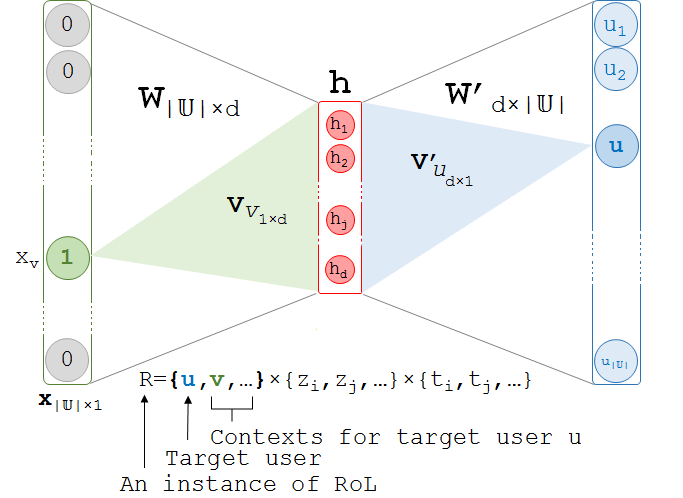
\includegraphics[width=0.8\columnwidth]{Images/neural_net.png}
\caption{The neural network architecture.\label{neural_net}}
\end{figure}

\subsubsection{User Embedding}
Given a set of discovered regions of like-mindedness (RoLs), the context for a user $u$ would be the set of users in each of the RoLs where $u$ had been observed. We formulate user vector learning as a maximum likelihood (ML) optimization problem. In particular, for each user, we find her like-minded users by optimizing the conditional probability of observing users that have the same RoLs as her. To induce the user embeddings, we adopt an approach similar to~\cite{DBLP:conf/nips/MikolovSCCD13} as follows:

\begin{definition}
\textbf{(Embedding Objective)} Given the set $\mathcal{R}$ of all regions of like-mindedness (RoLs), the embedding function $g:\mathbb{U}\rightarrow{[0,1]^d}$ maps each user $u\in\mathbb{U}$ onto a d-dimensional space, such that the following objective is optimized:
\begin{equation}\label{argmax}
    {\operatorname*{arg\,max}_g\sum_{R\in\mathcal{R},u\in{R}}{\text{log Pr}(u|R\setminus{u})}}
\end{equation}
\end{definition} 

In order to make the optimization tractable, we assume conditional independence for observing users in a RoL such as $R$. So, 
\begin{equation}\label{probability}
    \text{Pr}(u|R\setminus{u})=\prod_{v\in{R\setminus{u}}}{\text{Pr}(u|v)}
\end{equation} 
To learn the user embeddings, we use a single hidden layer, fully connected neural network. The architecture of our neural network is shown in Figure \ref{neural_net}. The hidden layer $\textbf{h}$ is of size $d$, the dimensionality of the resulting user vectors, and the input and output layer is set to have as many neurons as $|\mathbb{U}|$. Thus, the input to hidden layer connections can be represented by matrix $\textbf{W}$ of size $|\mathbb{U}|\times{d}$ with each row representing a vector for user $u\in\mathbb{U}$. The input layer $\textbf{x}$ is a one-hot encoded vector and the hidden layer's neurons are all linear such that $\textbf{h}=\textbf{W}^{\top}\textbf{x}$. Given a user $v$ in the input layer that is taken from the context of $u$, i.e., $u$ and $v$ have been observed in the same RoL, $\textbf{h}$ is the transpose of $v$'s corresponding row in $\textbf{W}$ named $\textbf{v}_v$. In the same way, the connections from hidden layer to output layer can be described by matrix $\textbf{W}'$ of size $d\times|\mathbb{U}|$. The prediction task could be done via a softmax function to approximate the probability of observing the target user $u$ given user $v$ from the same RoL, i.e.,

%In this case, the output layer value for the user $u$ is equal to $Y_u=(HO)_u$. 

\begin{equation}\label{softmax}
\text{Pr}(u|v) = \frac{\text{exp}({\textbf{v}'^{\top}_u\textbf{h}})}{\sum\limits_{w\in\mathbb{U}}{\text{exp}({\textbf{v}'^{\top}_w\textbf{h}})}}=\frac{\text{exp}({\textbf{v}'^{\top}_u\textbf{v}_v})}{\sum\limits_{w\in\mathbb{U}}{\text{exp}({\textbf{v}'^{\top}_w\textbf{v}_v})}}
\end{equation}
where $v'_u$ is $u$'s corresponding column of matrix $\textbf{W}'$. With the assumption in Equation \ref{probability} and the above probability function, the objective function in Equation \ref{argmax} simplifies to:
\begin{equation}\label{simplified_argmax}
{\operatorname*{arg\,max}_g\sum_{R\in\mathcal{R},u\in{R}}{\Big[\sum_{v\in{R}\setminus{u}}{\big[(\textbf{v}'^{\top}_u\textbf{v}_v)-\text{log}{\sum\limits_{w\in\mathbb{U}}{\text{exp}({\textbf{v}'^{\top}_w\textbf{v}_v})}}\big]} \Big]}}
\end{equation}


 %For each user $u\in\mathbb{U}$ there is a path $u_1,u_2,...,u_{h(u)}$ of height (length) $h(u)$ from the root, $u_1$, to her respective leaf, $u_{h(u)}$. This choice leads to speedup since similar users are accessed more quickly. 

%Hierarchical softmax defines $\text{Pr}(u|v)$ as follows:
%\begin{equation}
%\text{Pr}(u|v)=\prod_{i=1}^{h(u)-1}{s((-1)^{(u_{i+1} \stackrel{?}{=}child(u_i))}\times H_v\times O_{u_i}))}
%\end{equation}
%where $s(x)$ is the sigmoid function, $O_{u_i}$ is the vector representation for user $u_i$. $H_v\times O_{u_i}$ shows the similarity between the vector representation of user $v$ and the internal user $u_i$. At each internal user $u_i$, if we choose the left (right) child as the correct $u_{i+1}$ in the path from the root to the user's leaf, we have the probability $s((-1)^0x)=s(x)$, else the right(left) child would result in $s((-1)^1 x)=s(-x)$ such that $s(x)+s(-x)=1$. The intuition is that the more an output user $u$ is similar with the ancestors of input user $v$, the higher the probability would be that they are the same. 

Our neural network is trained using stochastic gradient descent and updates $\textbf{W}$ and $\textbf{W}'$ gradually via backpropagation. After the training converges, each row of $\textbf{W}$ represents the d-dimensional user embeddings. %A pair of like-minded users $u,v\in\mathbb{U}$ will, as a result, have highly similar vectors $\textbf{v}_u$ and $\textbf{v}_v$, accordingly.

\subsection{User Community Detection\label{community_detection}}
Given the user embeddings, we identify communities of users through graph-based partitioning heuristics. We represent users and their pairwise similarities through a weighted undirected graph. Precisely, let $\text{G}=(\mathbb{V},\mathbb{E}, s)$ be a weighted user graph in time period $\text{T}$ such that $\mathbb{V}=\mathbb{U},\mathbb{E}=\{e_{u,v}:\forall{u,v}\in\mathbb{U}\}$ and the weight function $s:\mathbb{E}\rightarrow[0,1]$ is the cosine similarity of embeddings for the incident users of an edge defined as $s(e_{u,v})=\frac{\textbf{v}_u\cdot{\textbf{v}_v}}{||\textbf{v}_u||_2||\textbf{v}_v||_2}$. After constructing the user graph G for a given time period T, it is possible to employ a graph partitioning heuristic to extract clusters of users that form latent communities. We leverage the Louvain method (LM)~\cite{1742-5468-2008-10-P10008} as it introduces linear heuristics to the problem of graph partitioning. The output is a set of induced subgraphs such as $\text{G}[\mathbb{C}]$ whose vertex set $\mathbb{C}\subset{\mathbb{V}}$ and edge set consists of all of the edges in $\mathbb{E}$ that have both endpoints in $\mathbb{C}$. Subgraph $\text{G}[\mathbb{C}]$ with $|\mathbb{C}|\geq2$ form an instance of \textit{temporal like-minded user community} assuming $\mathbb{C}\in\mathbb{P}^*$. The application of graph partitioning algorithms on G will produce temporal user communities $\mathbb{P}^*$ that consist of like-minded users who have contributed to the same topics with similar temporal behavior and contribution degrees.

\bibliographystyle{ACM-Reference-Format}
\bibliography{bibliography.bib} 

\end{document}

